%% IMPORTANT: Once working, run latex 3 times to get listoffigures to work

%% Be sure to check spelling!

%% Put **your** name and the proper due date in place

%% Copy the lstlisting and figure code as many times as you need
%% Be sure to put in your own file names if appropriate

%% Note that the \epsfig command is currently commented out - until the
%%%% files exist, processing this code without them will result in an error
%%%% so leave the comments until you have created the graphics files!

\documentclass{article}
\usepackage{amsmath}    % loads AMS-Math package
\usepackage{epsfig}     % allows PostScript files
\usepackage{listings}   % allows lstlisting environment
\usepackage{moreverb}   % allows listinginput environment
\usepackage[letterpaper, margin=0.75in]{geometry}  % set paper size/margins
\usepackage{textcomp}   % adds \interrobang, among others!

\begin{document}
\begin{center}
\rule{6.5in}{0.5mm}\\~\\
\textbf{\large EGR 103L -- Fall 2017}\\~\\
\textbf{\huge Laboratory 8 - Intermediate Curve Fitting}\\~\\
Ian Hanus (ih52)\\
Lab Section 1B, Tuesday 8:30-11:2-\\
November 12th, 2017\\~\\
{\small I have adhered to the Duke Community Standard in completing
  this assignment.  I understand that a violation of the Standard can
  result in failure of this assignment, failure of this course, and/or
  suspension from Duke University.} 
\rule{6.5in}{0.5mm}\\
\end{center}
\tableofcontents
\listoffigures
\renewcommand{\arraystretch}{1.5}
\clearpage

\section{Palm 6.9}
$S_T = 2.0361e+03$
\begin{center}
\begin{tabular}{|c|c|c|c|} \hline
Order & Coefficients $P$ of $T=f(A)=\sum_{k=1}^{\mbox{Order}+1}~P(k)A^{(\mbox{Order}+1-k)}$  & $S_r$ & $r^2$ \\ \hline
1 & [-6.9697e-01 1.0844e+02] & 1.9960e+03 & 1.9683e-02\\ \hline
2 & [-1.9053e+00 -1.7845e+01 1.3130e+02] & 7.9289e+01 & 9.6106e-01 \\ \hline
3 & [1.0684e-02 1.7611e+00 -1.7352e+01 1.3103e+02] & 7.8937e+01 & 9.6123e-01 \\ \hline
4 & [-2.4913e-02 4.5911e-01 -7.5510e-01 -1.2868e+01 1.2995e+02] & 6.8713e+01 & 9.6625e-01 \\ \hline
\end{tabular}
\end{center}
The minimum drying times and additive amounts for each fit are:
\begin{center}
\begin{tabular}{|c|c|c|} \hline
  Order & Min. Drying Time (min) & $A$ for Min. Drying
Time (oz) \\ \hline
1 & 8.9999e+00 & 1.0216e+02 \\ \hline
2 & 8.9518e+01 & 4.6829e+00 \\ \hline
3 & 8.9486e+01 & 4.7236e+00 \\ \hline
4 & 8.8304e+01 & 4.6765e+00 \\ \hline
\end{tabular}
\end{center}
% Discussion

\section{Palm 6.16}
\begin{align*}
y(x) = (5.7518e+00)+(9.9123e+00)\ln(x)
\end{align*}
The statistical information is:
\begin{align*}
S_t&=4.8359e+00 & S_r &= 3.0297e+03 & r^2 &=-6.2550e+02
\end{align*}
The estimates asked for using this model are:
\begin{align*}
y(2.5)&\approx 2.4292e+01  & y(11)&\approx 7.3182e+01
\end{align*}

\section{Chapra 15.7}
Based on the least-squares fit of the given models,
\begin{align*}
% replace PM with + or - as appropriate
OC(c,T)&=(1.4027e+01)-(1.4027e-01)-(3.3642e-01)T-(1.0493e-01)T^2+(1.4027e+01)T^3
\end{align*}
For this model with these data points, 
\begin{align*}
S_t &= 1.0400e+02 &
S_r &= 1.2784e+00 &
r^2 &= 9.8771e-01
\end{align*}
Because the $r^2$ value is so close to 1, above 0.95, this is model provides a good mathematical fit for the data.  The estimate of $OC(15,12)$ is 9.1678e+00 mg/L, which has a
relative error of (8.5605e-01)\% from the known value.

\section{Chapra 15.10}
Based on the least squares fit of the given model,
\begin{align*}
p(t)&= (4.1375e+00)e^{-1.5t} + (2.8959e+00)e^{-0.3t} + (1.5349e+00)e^{-0.05t}
\end{align*}
% Disccusion
The statistical and specific information required by the problem is:
\begin{center}
\begin{tabular}{|c|c|c|c|c|c|}\hline
$A$ & $B$ & $C$ & $S_T$ & $S_r$ & $r^2$ \\ \hline
$4.1375e+00$ & $2.8959e+00$ & $1.5349e+00$ & $2.0409e+01$ & $8.0348e-02$ & $9.9606e-01$\\ \hline
\end{tabular}
\end{center}
Because the $r^2$ value is so close to one, above 0.95, this model is a good mathematical fit for the data.

\section{Chapra 15.10 Alternate}
Based on the least squares fit of the given model,
\begin{align*}
p(t)&=(5.6328e+00)e^{-1.5t} - (4.4272e+00)e^{-0.3t}+ (7.8906e+00)e^{-0.2t}
\end{align*}
% Disccusion
The statistical and specific information required by the problem is:
\begin{center}
\begin{tabular}{|c|c|c|c|c|c|}\hline
$A$ & $B$ & $C$ & $S_t$ & $S_r$ & $r^2$\\ \hline
5.6328e+00 & -4.4272e+00  & 7.8906e+00 & 2.0409e+01 & 7.9611e-02 & 9.9610e-01 \\ \hline
\end{tabular}
\end{center}
Because the $r^2$ value is so close to one, above 0.95, this model is a good mathematical fit for the data.

\section{Chapra 15.12}
\begin{align*}
y(x) = (3.745e-01) + (9.8644e-01)x + \frac{8.4564e-01}{x}
\end{align*}
The statistical information is:
\begin{align*}
S_t&= 6.9480e+00 & S_r &=2.7651e-03  & r^2 &=9.9960e-01
\end{align*}
The estimates asked for using this model are:
\begin{align*}
y(1.5)&\approx 2.4179e+00 & y(4.5)&\approx 5.0014e+00
\end{align*}

\section{Chapra 15.11}
The model equation is:
\begin{align*}
P&=P_m\frac{I}{I_{sat}}e^{-\frac{I}{I_{sat}}-1}=
(2.3871e+02)\frac{I}{2.2182e+02}e^{-\frac{I}{2.2182e+02}-1}
\end{align*}
with $P_m$ measured in (mg m$^{-3}$ d$^{-1}$) and $I_{sat}$ measured in ($\mu$E m$^{-2}$s$^{-1}$).\\
\begin{center}
$S_r = 1.1159e+03 $\\     $S_t = 2.8370e+04$\\     $r^2 = 9.6067e-01$\\
\end{center}
Because the $r^2$ value is so close to 1, above 0.95, this model is a good mathematical fit for the data given. The initial guesses came from the maximum photosynthesis rate given in the tale and the I value that was near it.


\section{Chapra 15.14}
The $S_t$ for the data set is 1.0847e-09.  With a model of:
\begin{align*}
v_0=\frac{(2.4310e-05)[S]^3}{(3.9977e-01)+[S]^3}
\end{align*}
\begin{center}
$S_r = 2.1212e-18$\\     $S_t = 1.0847e-09$\\     $r^2 = 1.0000e+00$\\
\end{center}
Because $r^2$ is equal to one, this model is a perfect fit for the data. The initial guesses for $k_m$ and $S$ came from the limit of$v_0$ as S went to infinity and the $S^3$ value at about half of the $v_0$ maximu.

 
\pagebreak
\appendix
\section{Codes and Output}
% Put the name of your file in the subsection name 
% and the listinginput input
% Be sure to include the community standard in codes!
% Add \pagebreaks if they make sense
% Make as many copies as you need

\subsection{Paint.m}
\listinginput[1]{1}{Paint.m}

\subsection{Palm6p9.m}
\listinginput[1]{1}{Palm6p9.m}
\pagebreak

\subsection{Palm6p16.m}
\listinginput[1]{1}{Palm916.m}
\pagebreak

\subsection{Chapra15p7.m}
\listinginput[1]{1}{Chapra15p7.m}
\pagebreak

\subsection{Chapra15p10.m}
\listinginput[1]{1}{Chapra15p10.m}
\pagebreak

\subsection{Chapra15p10alt.m}
\listinginput[1]{1}{Chapra15p10alt.m}
\pagebreak

\subsection{Chapra15p12.m}
\listinginput[1]{1}{Chapra15p12.m}
\pagebreak

\subsection{Chapra15p11.m}
\listinginput[1]{1}{Chapra15p11.m}
\pagebreak

\subsection{Chapra15p14b.m}
\listinginput[1]{1}{Chapra15p14b.m}
\pagebreak



\section{Figures}
% Make as many as needed; change sizes if it makes sense to do so
\begin{figure}[h!]
\begin{center}
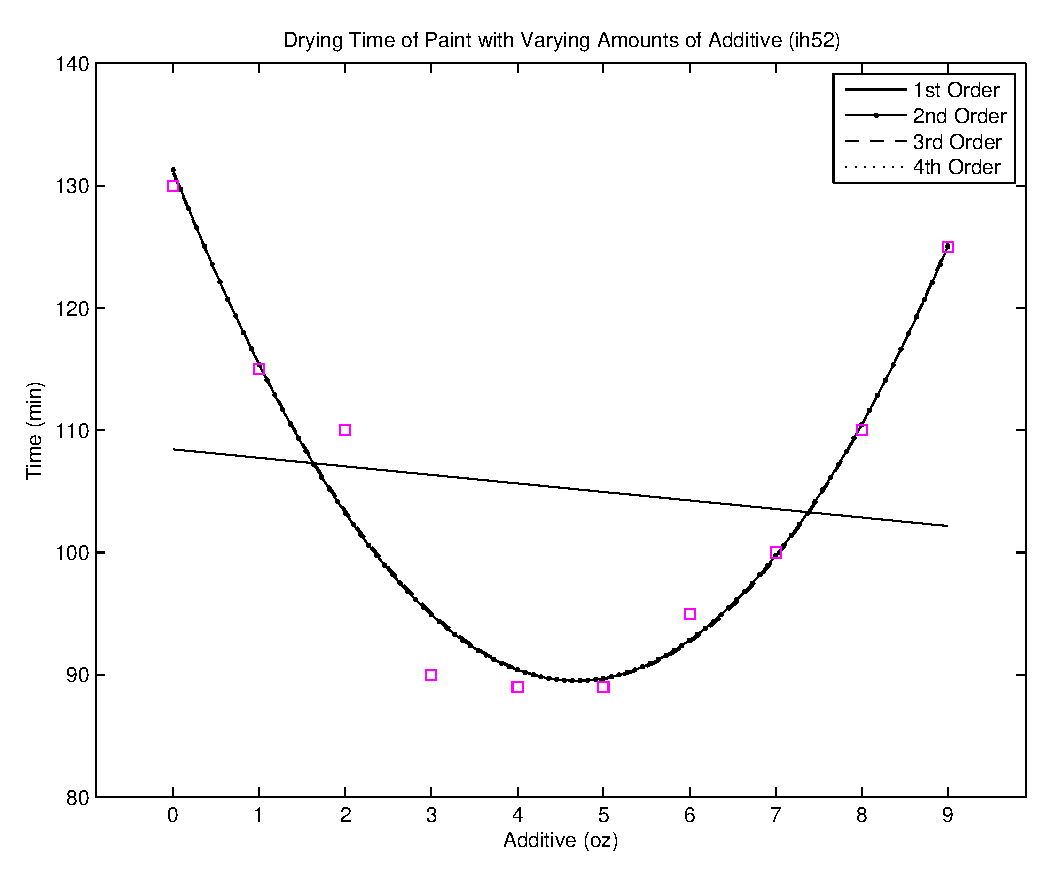
\epsfig{file=Palm6p9plot.eps, width=3in}
\caption{Palm 6.9}
\end{center}
\end{figure}

\begin{figure}[htb!]
\begin{center}
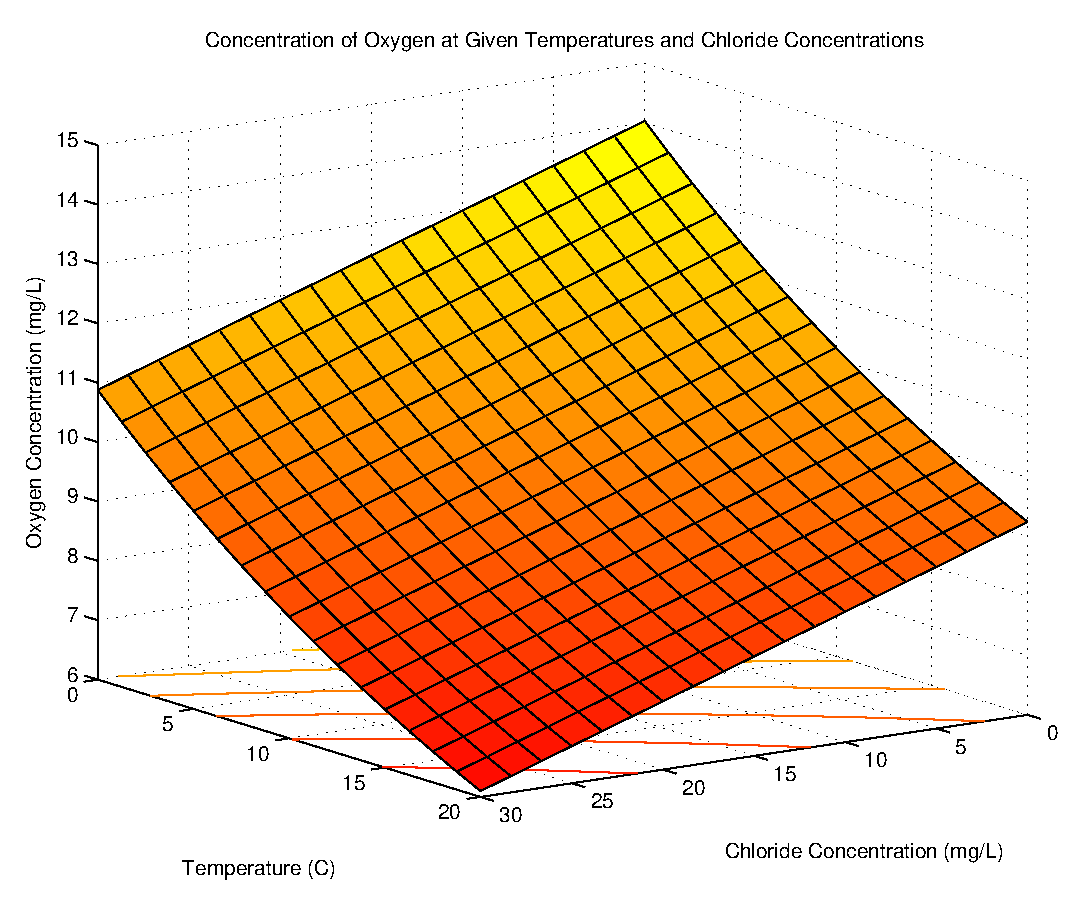
\epsfig{file=Chapra15p7plot.eps, width=4in}
\caption{Chapra 15.7}
\end{center}
\end{figure}
\clearpage

\begin{figure}[htb!]
\begin{center}
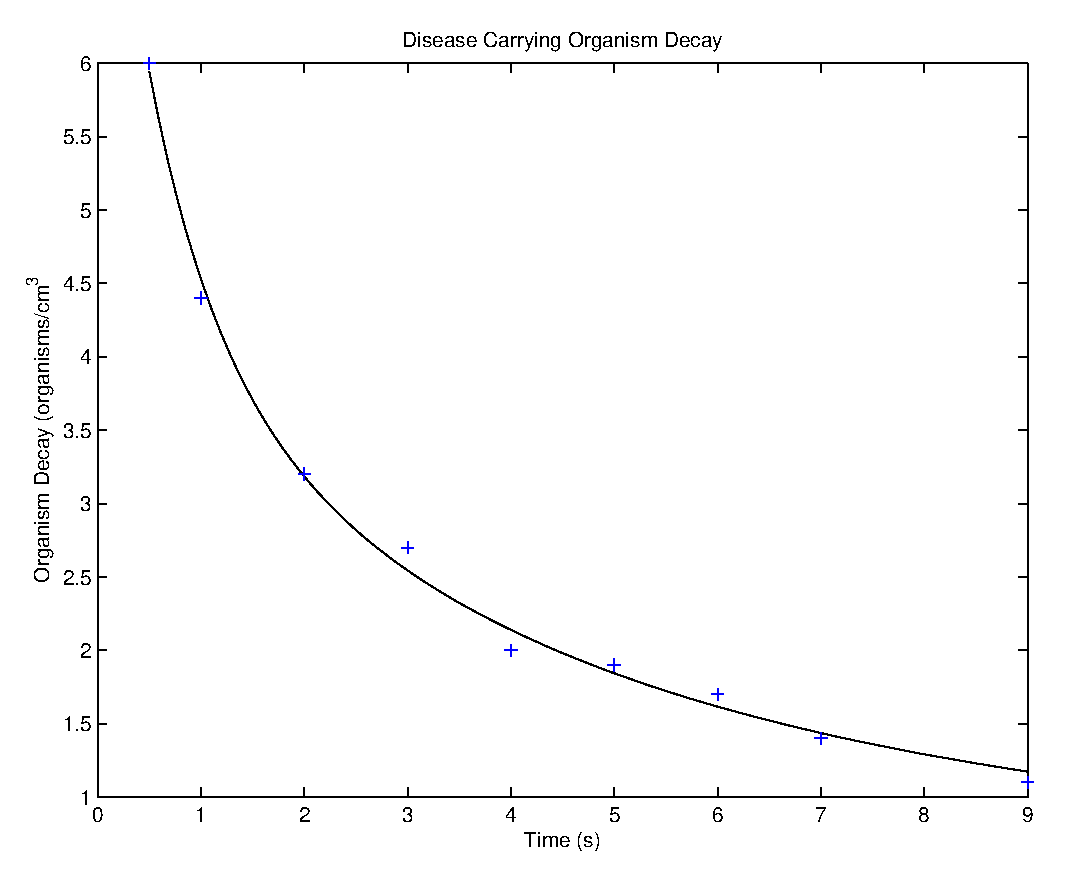
\epsfig{file=Chapra15p10plot1.eps, width=3.in} ~
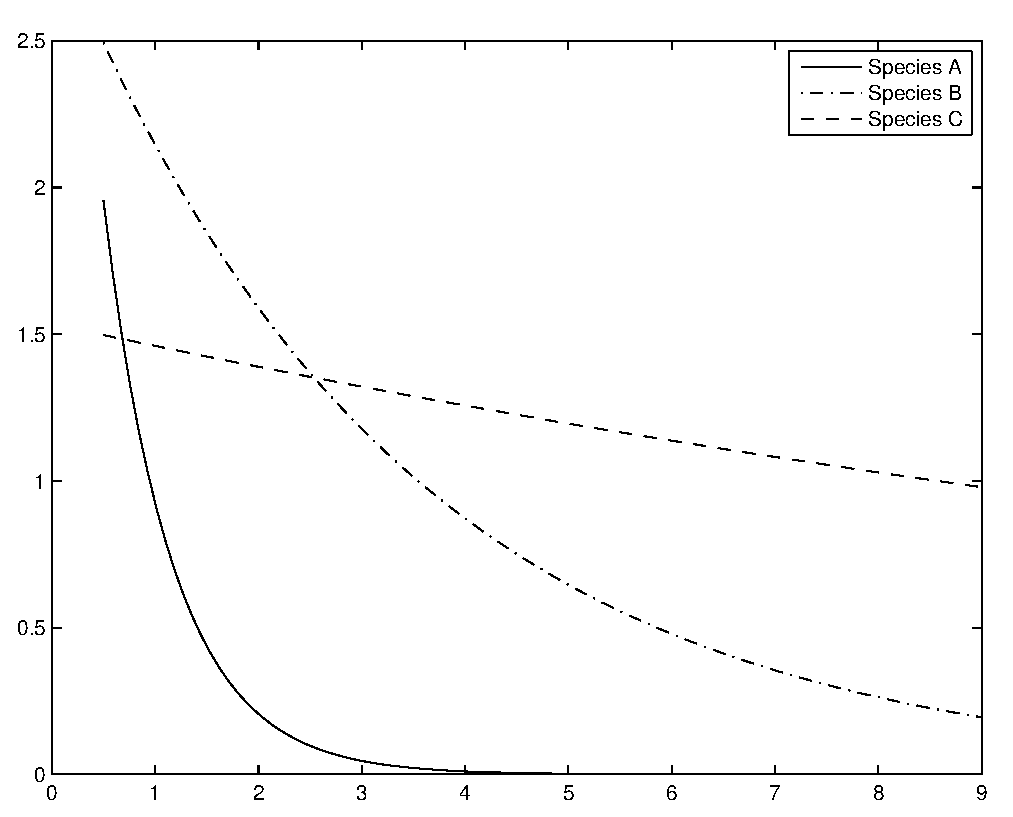
\epsfig{file=Chapra15p10plot2.eps, width=3.in}
\caption{Chapra 15.10}
\end{center}
\end{figure}

\begin{figure}[htb!]
\begin{center}
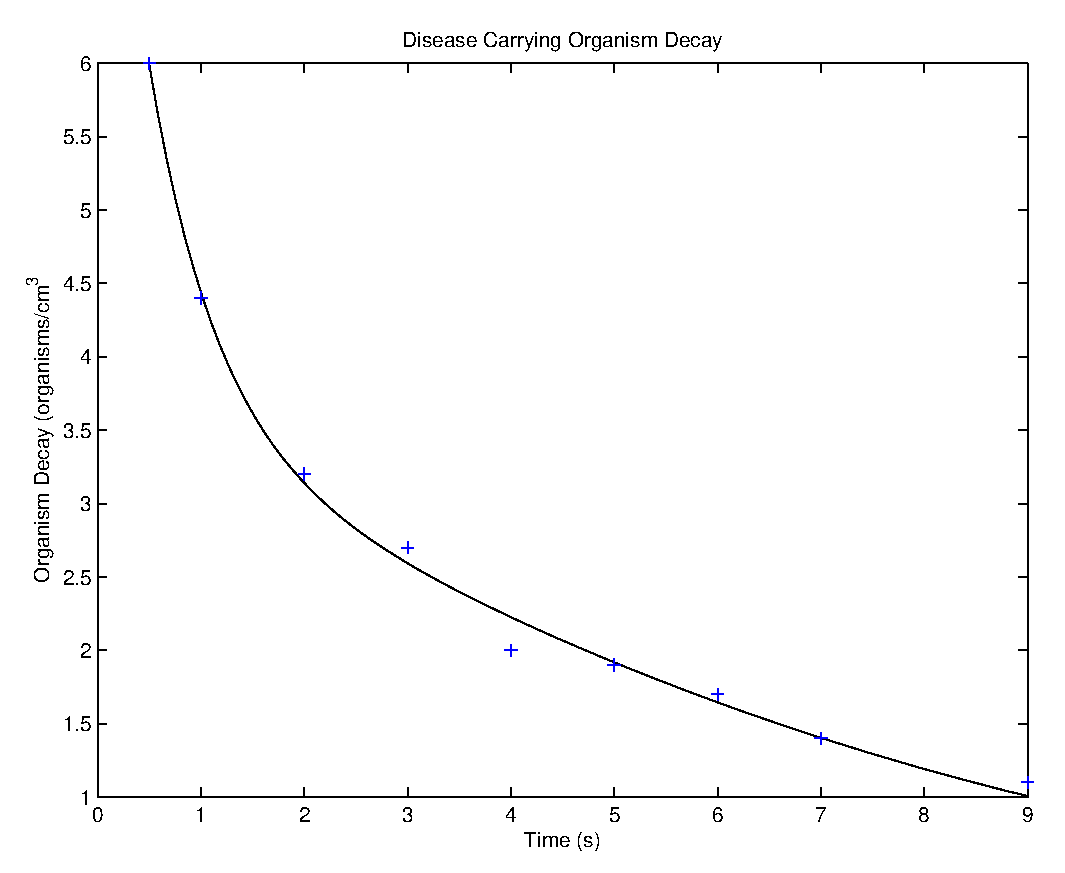
\epsfig{file=Chapra15p10altplot1.eps, width=3.in} ~
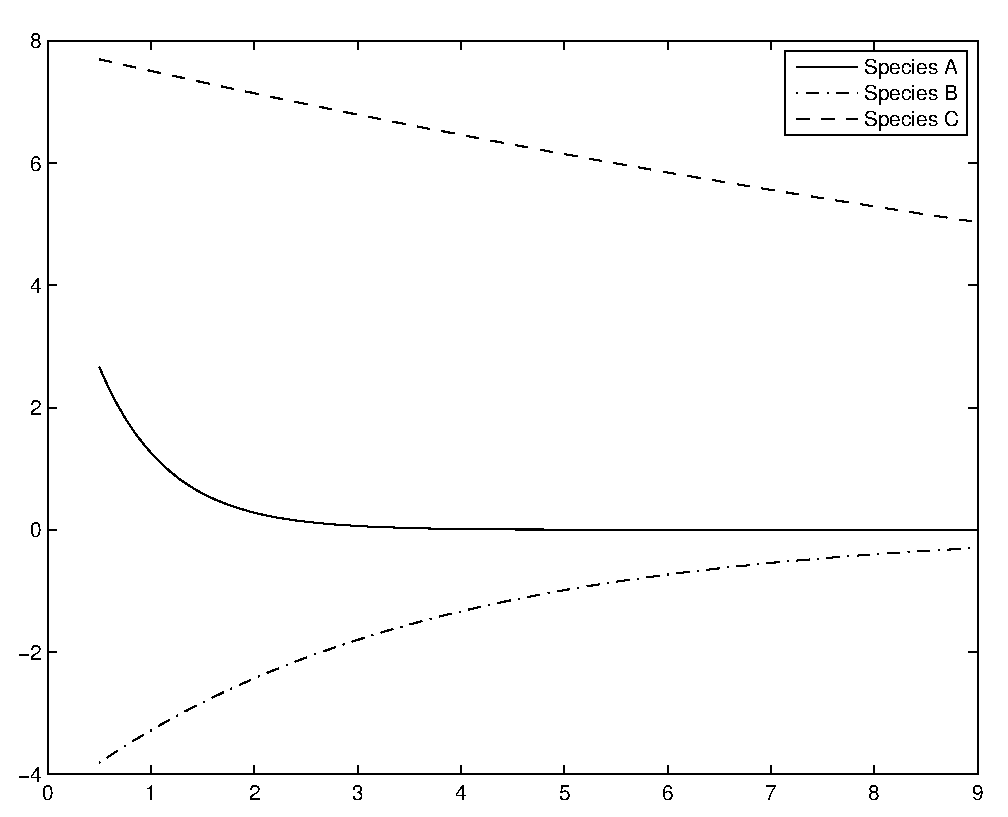
\epsfig{file=Chapra15p10altplot2.eps, width=3.in}
\caption{Chapra 15.10 Alternate}
\end{center}
\end{figure}
\clearpage

\begin{figure}[htb!]
\begin{center}
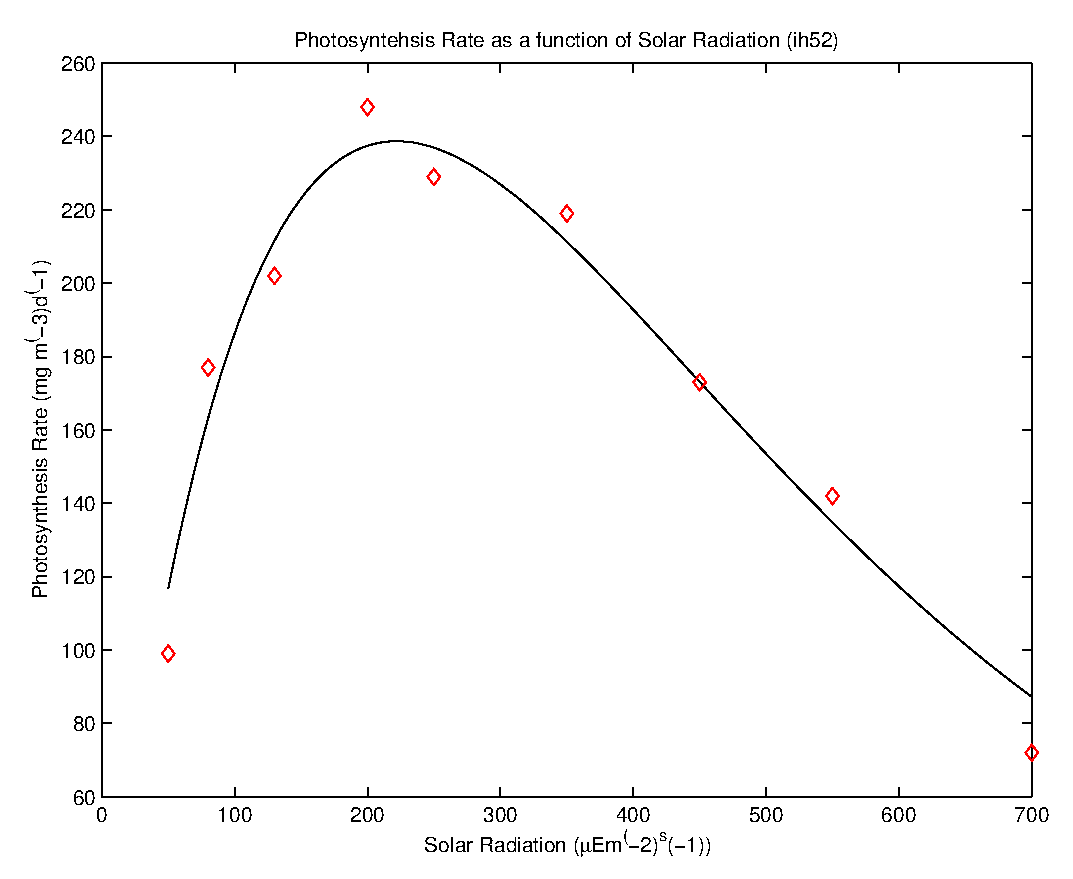
\epsfig{file=Chapra15p11plot.eps, width=4in}
\caption{Chapra 15.11}
\end{center}
\end{figure}

\begin{figure}[htb!]
\begin{center}
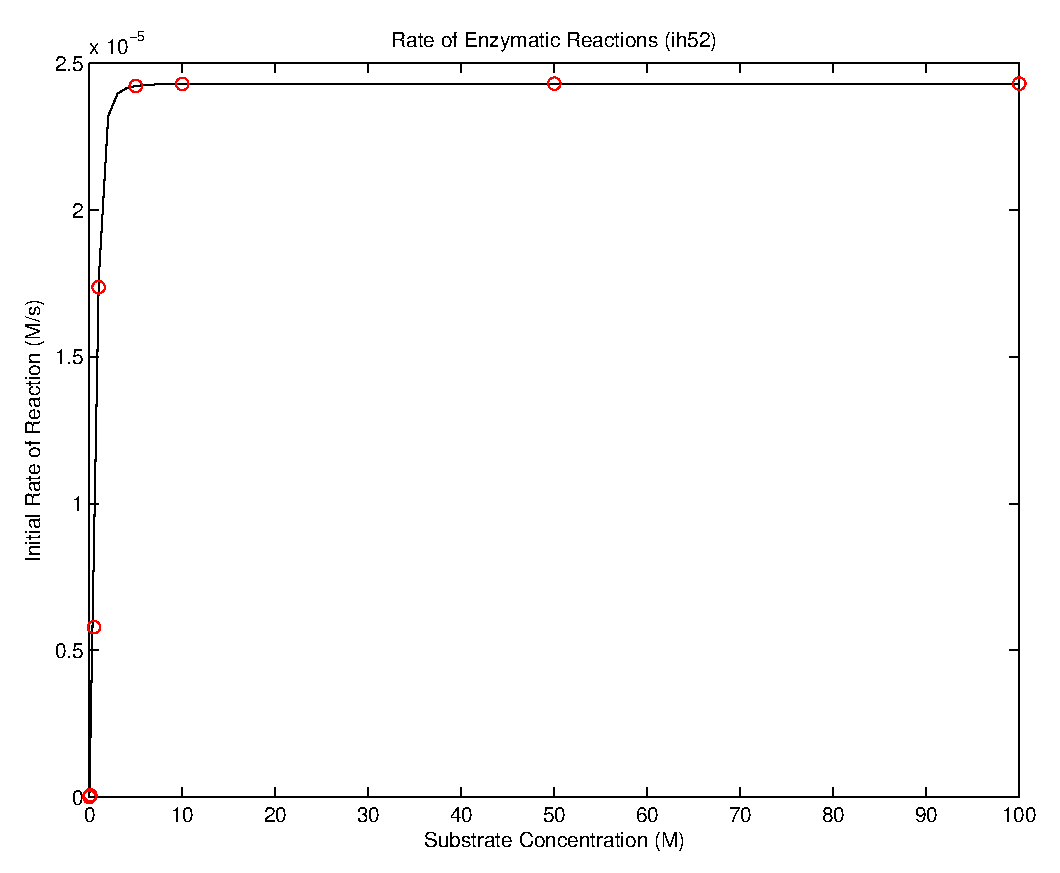
\epsfig{file=Chapra15p14bplot.eps, width=3.1in} ~
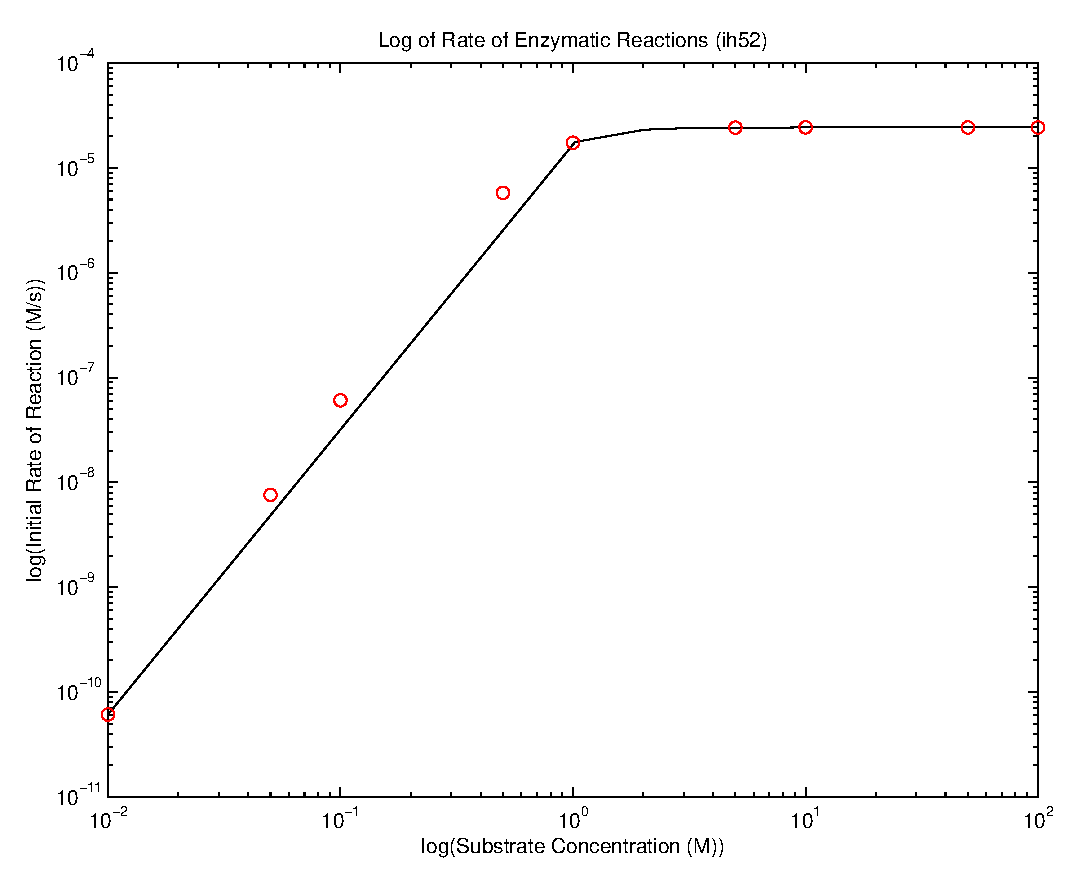
\epsfig{file=Chapra15p14blogplot.eps, width=3.1in}
\caption{Chapra 15.14}
\end{center}
\end{figure}

\end{document}

% LocalWords:  
